
\subsection{Steps to a solution}
\begin{itemize}
    \item Create a new low level file, call it: \textit{circular\_shift\_register.sv}.
    \item This new module should output 16, 8-bit registers. These will be the duty cycles of the PWM modules.
    \item On reset each of these 8-bit registers should be instantiated with different values: 0,0,0,0,16,32,64,256,256,64,32,16,0,0,0,0 makes for reasonable values.
    \item On each clock cycle, the registers should shift one over, similar to a shift register; except, the last register shifts into the first register.
    \item Write a test bench and observe the outputs cycling.
\end{itemize}
\subsubsection{Creating the Circular Shift Register}
To create the shift register module press the plus button on the sources window similar to how we added sources previously. However, instead of selecting add file select create file.
\begin{figure}[H]
    \centering
    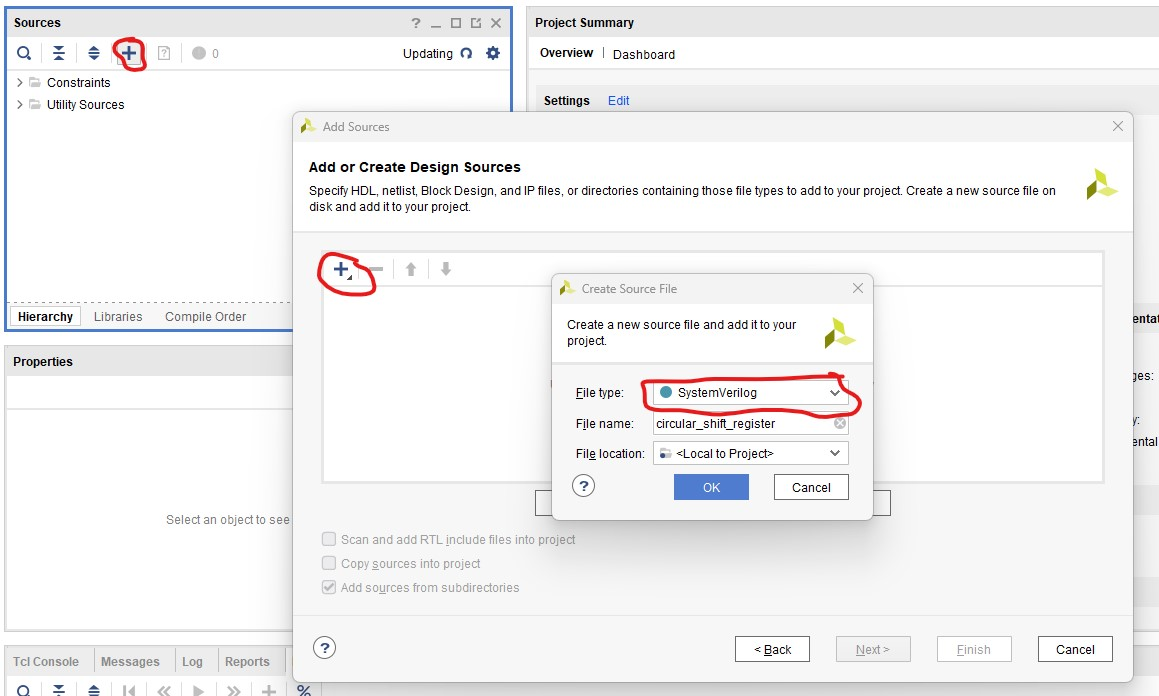
\includegraphics[width=9cm]{Images/CreateFile/create_system_verilog_file.jpg}
    \caption{Create a System Verilog File}
    \label{fig:enter-label}
\end{figure}
\begin{itemize}
    \item Select the Plus in the Sources Window
    \item Select "Add or create design sources"
    \item Select the Plus in the wizard window
    \item Select "Create File..."
    \item Give the file a name: \textit{circular\_shift\_register}. And be sure to select System Verilog.
    \item Select Finish
\end{itemize}
\begin{figure}[H]
    \centering
    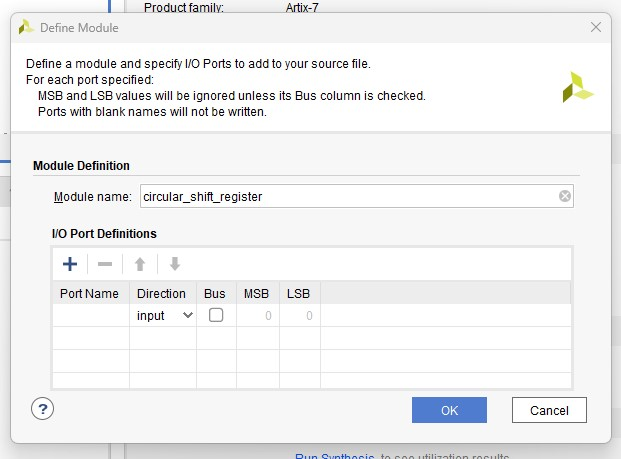
\includegraphics[width=9cm]{Images/CreateFile/DefineModule.jpg}
    \caption{Define Module Window}
    \label{fig:enter-label}
\end{figure}
The define module window will pop up. This defines the input and output ports for the module being designed. Add the ports to the window to produce the following ports. Select bus and adjust MSB to create ports of more than one bit.
\begin{itemize}
    \item Create an input port named clk,
    \item Another Input port named rst\_n,
    \item And finally an output port named reg\_out, make it a bus and make it 128 bits wide (This means the MSB is 127, not 128!)
\end{itemize}
Opening up your module you should see the following:
\begin{verbatim}
    module circular_shift_register(
    input clk,
    input rst_n,
    output [127:0] reg_out
    );
endmodule
\end{verbatim}
The very long register as it is created here will be difficult to work with. Therefore we want to change it to a packed array of 16 8-bit registers. To this end change the register out to be:
\begin{verbatim}
    output logic [7:0] reg_out[15:0]
\end{verbatim}
Now with that setup we can start by declaring the register internally.
\begin{verbatim}
    logic [7:0] circ_reg [15:0];
    assign reg_out = circ_reg;
\end{verbatim}
While we could work directly with the output register instead of having this internal declaration it can be good practice to split it like this as in larger designs it can allow for additional layers of abstraction or for hiding internal states when working with more complicated designs.

\begin{lstlisting}

// Always block triggered by a positive edge of the clock
always_ff @(posedge clk) begin
    if (!rst_n) begin
        // Reset the register array to the initial state
        circ_reg <= ??
|\colorbox{magenta!30}{// Assign appropriate reset values to every element of the circular shift register}|
    end else begin
        // Circularly shift the register array
        circ_reg <= ??
|\colorbox{magenta!30}{// Create the circular shifting register behavior}|
    end
end
\end{lstlisting}

You'll need to create a synchronous reset which will set the value of each 8-bit register in circ\_reg, then on every clock cycle you'll need to create a shift register behavior where the last value in the register becomes the first. Once you believe you have this you'll need to create a new file for the test bench.\\

This module is simple enough that you can practically test every possible state by declaring the device under test, resetting the registers to bring them into known states, and running through the clock 16 times to cycle through all possible values. You can also be much more creative with the test bench if you so choose.

\begin{lstlisting}
module tb_circular_shift_register;

    // Parameters
    parameter WIDTH = 8;
    parameter SIZE = 16;

    // Clock and reset signals
    logic clk;
    logic rst_n;

    // Output array for observing the register state
    logic [WIDTH-1:0] reg_out[SIZE-1:0];

    // Instantiate DUT
    circular_shift_register u_circular_shift_register (
        .clk(clk),
        .rst_n(rst_n),
        .reg_out(reg_out)
    );

    // Clock generation
    always begin
        #5 clk = ~clk; // 10 time unit period
    end

    // Testbench stimulus
    initial begin
        // Initialize signals
        clk = 0;
        rst_n = 0;
        
        // Apply reset
        #10 rst_n = 1;

        // Loop through 16 cycles and print the register state
        repeat (SIZE) begin
            #10; // Wait for one clock cycle
            $display("Register State:");
            $display("reg_out[0] = %h",reg_out[0]) ;
            ... ...
        end

        // Finish the simulation
        $finish;
    end

endmodule
\end{lstlisting}
You can use this to test your circular shift register. You will potentially want to add some additional code to improve the test bench. You can add checks to confirm that it is indeed circling, or you can manually observe the behavior in the waveform window. 
\subsubsection{Create Top Level}

With the test bench and this module complete you have the minimum needed number of lower level cells. You could decide to make a specialized cell for clock division, or you can reuse the PWM module with appropriate values to produce a slow clock. You need this slower clock to drive your circular shift register so that you can visualize the patterns being created. You can use the provided PWM test bench to find a good maximum value, and duty cycle through trial and error or deliberate calculation. \\
\vspace{0.5cm}
For the top level:
\begin{itemize}
    \item Instantiate 16 copies of the PWM module. Hook one PWM module up to each LED output. 
    \item Instantiate 1 copy of your circular shift register. Hook each PWM duty cycle up to one of the output registers. 
    \item Instantiate either an appropriately configured PWM module, or a dedicated clock divider to produce a slow clock for the circular shift register. 
    \item Modify the provided top level test bench and produce the needed text file to run through the python web application to verify your results visually. 
\end{itemize}
Extend the LED Output on the top module.
\begin{verbatim}
    output reg [15:0] led
\end{verbatim}
Declare 16 copies of the PWM Module
\begin{verbatim}
    pwm_module #(
        .bit_width(bit_width)
    ) pwm_unit (
        .clk(clk),
        .rst_n(rst_n),
        .duty(duty[i]),
        .max_value(8'd255),
        .pwm_out(pwm_out[i])
    );
\end{verbatim}
For these modules we are going to want a bit width of 8 bits to match with the circular shift register we created, and then we are going to set our maximum value to 255. duty[i] is going to be outputs from the circular shift register and will be 0 to 15. We will need to declare the associated logic to hook up from the pwm modules to the circular shift register. Finally pwm\_out is going to be directed towards the 16 led outputs. \\

Let's declare the variables to hook everything together.
\begin{verbatim}
    logic rst_n;
    logic [7:0] duty [15:0];
    logic [15:0] pwm_out;
    // Output of the circular shift register
    logic [7:0] reg_out [15:0]; 
    // Reduced clock signal for the circular shift register
    logic clk_reduced; 
\end{verbatim}

You can see here I have declared rst\_n. This is because I have added this line to the top module.
\begin{verbatim}
    assign rst_n = ~reset;
\end{verbatim}
This is technically breaking the rule of no logic on the top level of a design. But this can be considered the absolute most that is acceptable, even if it is frowned upon. If you want to adhere to absolute best practices, create an additional module which will take a reset input, and deliver rst, and rst\_n outputs. These outputs may be generated through either combinational or sequential logic. In larger designs appropriate handling of reset can become a significant challenge. 

\begin{verbatim}
    circular_shift_register csr (
        .clk(clk_reduced),
        .rst_n(rst_n),
        .reg_out(reg_out)
    );
\end{verbatim}

Declare your circular shift register. You'll notice that I'm feeding it a reduced clock speed. If cycling at the 100MHz clock cycle it would loop around every 160ns, even if the pwm module were running fast enough to reflect this it is far too fast for our eyes to see. Next you'll want to declare an additional PWM module to generate your output values. 

\begin{verbatim}
        pwm_module #(
        .bit_width(?) 
    ) clk_reducer (
        .clk(clk),
        .rst_n(rst_n),
        .duty(?), 
        .max_value(?),
        .pwm_out(clk_reduced)
    );
\end{verbatim}

Find appropriate values for duty, max\_value, and bit\_width to create a visible cycling of the led brightness.\\
\vspace{1cm}
Lastly \textbf{remember} to add appropriate assigns to connect the circular shift register to the pwm modules, and the pwm outputs to the leds. With this complete create a new top level test bench to verify the behavior. 

\subsubsection{Top Level Test bench}
You can reuse the old top level test bench. With a few minor changes. 
\begin{itemize}
    \item Remove the switch adjusting behavior and simply wait a long period of time after the reset is complete.
    \item Modify the print to file function call to pass all the led values. Removing the zeros and replacing them with the led values. \begin{verbatim}
        print_leds_to_file({led,15'b000000000000000}, file_descriptor);
    \end{verbatim}
\end{itemize}

Run your simulation again, this will take 5 - 20 minutes. Afterwards your led.txt will contain lines like this:
\begin{verbatim}
    0.0000150000 0000000000000000
    0.0000450000 1111111111111111
    0.0000550000 0000011111111000
    0.0002150000 0000001111110000
    0.0003750000 0000000111100000
    0.0006950000 0000000011000000
\end{verbatim}
The timing will be different and will shift as you progress through the very long file. You can then produce a video representation to confirm you have a good led pattern using the same online tool as for the original design. 

\begin{figure}[H]
    \centering
    
\includegraphics[height=1cm]{Images/ProvidedPWM/FinalOutput.jpg}
    \caption{Generated Video Output}
    \label{fig:enter-label}
\end{figure}
